\documentclass{article}
\usepackage[utf8]{inputenc}
\usepackage{graphicx}

\title{Perchè EA}
\author{Cecca Francesco Pio}
\date{October 2021}

\begin{document}

\maketitle

\section{Rettificatori}

\textbf{Perchè quando sono accesi D1 e D3, D2 e D4 sono spenti? } \\
Perchè la tensione su D2 e D4 sarebbe negativa, di conseguenza per un diodo ideale si avrà un circuito aperto. \\ \\
\textbf{Perchè devo aggiungere un low-pass per migliorare le prestazioni del mio rettificatore?} \\
Perchè voglio produrre una tensione più continua possibile (con l'onda raddrizzata ci sono ancora troppe oscillazioni) \\ \\
\textbf{Come funziona un raddrizzatore con filtro?} \\
Supponiamo il condensatore inizialmente scarico (tensione ai suoi capi nulla). Il condensatore si carica durante la semionda positiva dell'onda di ingresso (quando il diodo è polarizzato direttamente). La sua carica (e dunque la tensione ai suoi capi) raggiunge il valore massimo in corrispondenza del massimo dell'onda. \\
Quando la tensione del generatore comincia a scendere, il condensatore "vorrebbe" scaricarsi. Tuttavia non può scaricarsi attraverso il diodo, poiché quest'ultimo impedisce il passaggio della corrente in quella direzione. In pratica il diodo si trova a essere polarizzato con una tensione sul catodo maggiore di quella presente sull'anodo: entra dunque in polarizzazione inversa. \\
Ciò ha l'effetto di "isolare" il gruppo RC dal resto del circuito: durante la semionda negativa, il condensatore si scarica sulla resistenza R. Il tempo di scarica dipende dal valore della costante di tempo del gruppo RC (tau = RC) e l'andamento della scarica è il tipico esponenziale decrescente. \\
Il diodo ricomincia a condurre (torna in polarizzazione diretta), solo quando la tensione del generatore supera la tensione sul condensatore. A questo punto il condensatore torna nuovamente a caricarsi fino al valore massimo e il processo si ripete allo stesso modo nei periodi successivi. \\
L'effetto finale è quello di produrre una tensione che, pur non essendo ancora "continua", ha oscillazioni molto minori dell'onda raddrizzata di partenza. In generale le ondulazione residue (dette ripple) sono tanto minori quanto maggiore è il valore della costante di tempo tau = RC del gruppo RC.

\section{Amplificatori Differenziali}

\textbf{Come ottengo gli specchi di corrente?} \\
Una corrente di riferimento di ingresso è applicata al BJT collegato come diodo, determinando una tensione base-emettitore (VBE1) adeguata a IB1.
\begin{center}
    Ir={Vcc-Vbe/R}
\end{center} 
La tensione di base-emettitore (VBE2) del transistor TR2 viene forzata ad uguagliare VBE1.
\begin{center}
    Ir={Ib1+Ib2+Ic1}  
\end{center}
Supponendo i due transistors identici, da VBE1 = VBE2 ne discende che IB1 = IB2 e IC1 = IC2 = I2, e tenendo presente la relazione in zona di funzionamento lineare fra correnti di base e di collettore IB = IC/b , i ha: 
\begin{equation}
    Ir=2Ib+Ic2=Ic2+2\cdot\frac{Ic2}{\beta} = \frac{\beta + 2}{\beta}\cdot Ic2 
\end{equation}
Dalla quale ricaviamo 
\begin{equation}
    Ic2\equiv{\frac{\beta}{\beta+2}\cdot Ir} \Rightarrow \beta >> 2 \Rightarrow Ic2={Ir}
\end{equation} \\
\textbf{PROBLEMA: Range di tensione} \\
Dipende, nel caso di specchi a MOSFET, dalla condizione che i 2 transistor siano in saturazione.
\begin{equation}
    v \geq v_{ds_{sat}}
\end{equation}
Quindi se la v cresce o scende, passa dalla saturazione al triodo/sottosoglia e quindi cambia la formula della corrente. Di conseguenza lo specchio non specchia più. \\ 
Per capire meglio analizzare la figura a pagina 3 \\ \\
\textbf{PROBLEMA: I deve essere più costante possibile al variare di v }\\
Questo perchè la R{o} è la R di Norton del generatore di corrente.
Se voglio usarlo in un amplificatore differenziale, R{o}  deve essere la più grande possibile affinchè il rumore diminuisca 

\subsection{Amplificatori Differenziali con Carico Attivo}
Gli specchi di corrente possono essere usati nell'amplificatore differenziale, oltre che per implementare il generatore di correrne di polarizzazione, anche per sostituire le R.\\
Dato che $i_{C_{3}}=i_{C_{4}}$ e $i_{c_{1}}=-i_{c_{2}}$ in AC
$i_{0}=i_{c_{4}}-i_{c_{2}}=i_{c_{3}}+i_{c_{1}}\simeq2i_{c_{1}}=g_{m}v_{d}$ \\
\begin{center}
    $2i_{c_{1}}=g_{m}v_{d}$  e  $\frac{v_{o}}{v_{d}}=g_{m}R_{L}$
\end{center}

\newpage

\section{Comportamento in Frequenza}

\textbf{Metodo delle costanti di tempo}\\
Il metodo delle costanti di tempo a circuito aperto si usa per il calcolo dei coefficienti $b_{i}$ delle f.d.r così fatte:
\begin{equation}
    H(s)=\frac{1}{1+b_{1}s+b_{2}s^2+...+b_{n}s^n}
\end{equation}
Questa è una funzione LOW PASS, senza zeri o a frequenze così alte da essere trascurati.\\
Isolo i C in modo da rimanere con una rete A composta da elementi senza memoria.\\
Pongo il $det[Y]=0$ in modo da ottenere le frequenze naturali (poli del circuito).
\begin{equation}
    det[Y]=1+\sum b_{i}s^i
\end{equation}
Si è dimostrato che :
\begin{equation}
    b_{i}=\sum R_{i}C_{i} = \sum \tau_{i} => \omega_{H}=\frac{1}{b_{i}}=\frac{1}{\sum \tau_{i}}
\end{equation}
Per applicare il metodo delle costanti di tempo la $H_{H}$ deve essere scritta come la H(s) di sopra.\\
Quindi i condensatori che introducono uno zero prima del polo non vanno aggiunti nel metodo delle c.d.t per la stima della $\omega_{H}$\\
Per decidere si usa un generatore di test: se una volta cortocircuitato il C in esame, il guadagno diminuisce, allora il C va aggiunto, mentre se aumenta, non va considerato.\\
Viceversa per il metodo delle costanti di tempo a corto circuito.\\\\
\textbf{Quali condensatori usare?} \\
Analizzo prima quali condensatori usare per il \textbf{metodo a circuito aperto}.\\
Considerare, alle medie frequenze, che tutti i boli e gli zeri alle basse frequenze hanno già fatto effetto, equivale a considerare che tutti i condensatori responsabili di questi poli e zeri come cortocircuiti. \\ Quindi, la rete che corrisponde alla $ H_{h} $ (che lavora ad alte frequenze), è un amplificatore in AC con tutti i C di blocco/bypass cortocircuitati e con in evidenza i condensatori parassiti, i quali lavorano ad alte frequenze. \\
Analizzo, ora, quali condensatori usare per il \textbf{metodo a cortocircuito}.\\
Per il calcolo della $ \omega_{L} $
so che devo lavorare a basse frequenze e quindi avrò l'opposto di prima.\\ Quindi avrò che agiranno i C di blocco/bypass, mentre i C parassiti saranno circuiti aperti.
\newpage
\noindent
\textbf{Qual è il problema dell'EC?} \\
Analizzando e confrontando le $ \tau $ delle 3 configurazioni, noto che nell'EC le $ \tau $ sono molto più grandi e questo è un problema perchè, dal metodo delle costanti di tempo, so che la frequenza di taglio è l'inverso della somma delle $ \tau.$ \\
Quindi, avere costanti di tempo grandi, comporta una frequenza di taglio superiore bassa e quindi una banda più stretta e questo è un problemone perchè avere una banda stretta può causare distorsione del segnale che transita attraverso l'amplificatore, se questo ha delle componenti dello spettro a frequenza maggiori della frequenza di taglio superiore. \\ \\
\textbf{Collettore Comune - Emettitore Comune}\\
Sostituisco la $R_{S}$ di EC con la R d'uscita del CC.
Posso stare tranquillo che $\tau$ addizionali non vanificheranno il vantaggio ottenuto dalla diminuzione della $R_{i}$, data la alta frequenza di taglio della configurazione.\\
Il guadagno totale di tensione sarà circa uguale al guadagno di EC $A_{v_{EC}}$  dato che il CC ha $A_{v}=1$ se caricato da una R molto alta.\\\\
\textbf{Figura relativa ai problemi negli specchi di corrente:}
\vspace{0.8mm}
\begin{center}
    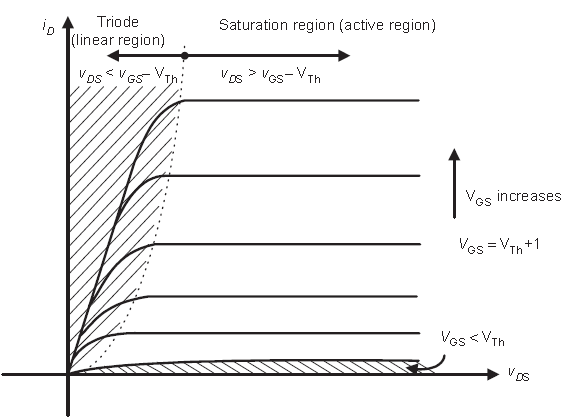
\includegraphics[scale=0.8]{Mosfet.png}
\end{center}

\newpage
\section{Retroazione}

\textbf{Come realizzo una retroazione positiva?} \\
Basta collegare la retroazione sul più, invece che sul meno, e questo comporterà il cambio si segno di $
    A(\omega)\beta $ \\ \\
\textbf{Analizzo la stabilità} \\
Per 1/2 poli è sempre verificata, mentre per 3 no perchè posso avere poli a Re>0 \\
Studio la stabilità con il criterio di Nyquist \\
\begin{equation}
    N=Z-P
\end{equation}
dove N è il numero di giri attorno a (-1,0), Z è il numero di zeri a Re>0 e P è il numero di poli a $
    Re>0
$ (risulterà P=0 perchè voglio studiare la stabilità e quindi non voglio poli a $
    Re>0
$.\\
Quindi la condizione di stabilità diventa:
\begin{equation}
    Z=0 => N=0
\end{equation}
Dalla definizione di stabilità regolare, cioè con una sola intersezione con il semiasse negativo, posso passare a Bode con condizioni ricavate osservando Nyquist.
\begin{enumerate}
    \item $ |A\beta(\omega_{\pi})|<1 ,   \phi(\omega_{\pi})=-\pi $
    \item $|A\beta(\omega_{t})|=1 ,   |\phi(\omega_{t})|<\pi$
\end{enumerate}
Se voglio graficare solo $A(\omega)$ si ha:
\begin{enumerate}
    \item $ |A(\omega_{\pi})|<\frac{1}{|\beta|} $ quando $ \phi(\omega_{\pi})=-\pi$
    \item $|A(\omega_{t})|=\frac{1}{|\beta|} $  quando $ |\phi(\omega_{t})|<\pi$
\end{enumerate}
\vspace{4mm}
\begin{center}
    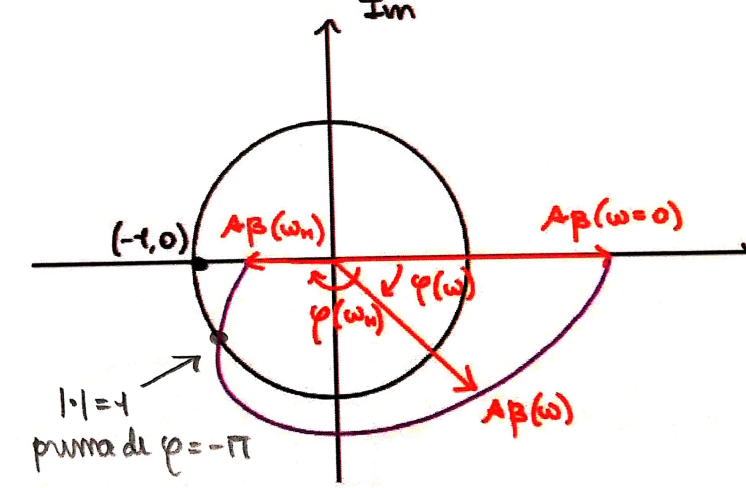
\includegraphics[scale=0.6]{Nyquist.png}
\end{center} 
\vspace{4mm}

\newpage
\noindent
Se $\frac{1}{\beta}=A_{F}$ fosse più basso, l'incrocio avverrebbe dopo. (vedi figura)
Quindi l'incrocio con $\frac{1}{\beta}$ deve avvenire prima di $\omega_{H}$ e per fare ciò potrei aver bisogno che $\frac{1}{\beta}=A_{F}$ sia molto alto. Se voglio un guadagno qualunque bisogna modificare l'amplificatore.
\begin{itemize}
    \item introduzione di un polo a low frequenza
    \item spostamento indietro del primo polo ottenuta aggiungendo una C a bassa frequenza
\end{itemize}
La seconda opzione, ovviamente è la migliore perchè aumenta la banda (1 decade in più) \\
\vspace{4mm}
\begin{center}
    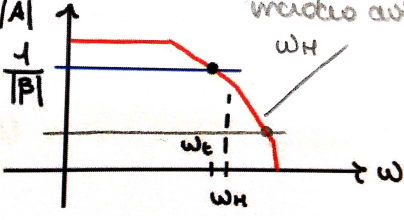
\includegraphics[scale=1]{Bode.png}
\end{center}
\vspace{4mm}
\subsection{ROC}
La stabilità può essere studiata con il margine di fase attraverso la \textbf{ROC}.
\begin{equation}
    \mbox {ROC = pendenza di} \frac{1}{\beta} - \mbox{pendenza di }A(\omega) 
\end{equation}
\begin{equation}
    \phi_{M}=180°-\frac{9}{2}ROC
\end{equation}

\newpage
\section{Amplificatori Operazionali}
\textbf{Zone di funzionamento}
\begin{enumerate}
    \item Zona lineare: $v_{+}=v_{-}$
    \item Zona di saturazione positiva: $v_{o}=V_{DD}$ (valida solo se $v_{+}>v_{-}$)
    \item Zona di saturazione negativa: $v_{o}=-V_{DD}$ (valida solo se $v_{+}<v_{-}$)
    \end{enumerate}
\begin{center}
    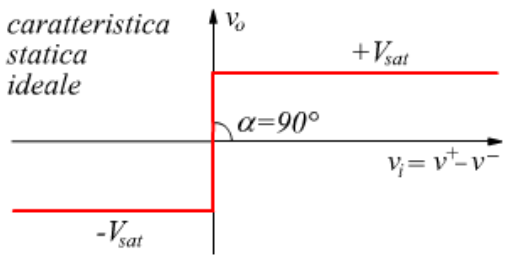
\includegraphics[scale=0.7]{Opamp.png}
\end{center}
\subsection{Modello di Gilbert}
L'idealità dell'OPAMP,, cioè del nullore, si può collegare con la figura di merito del $GBW=A_{f}\omega_{H_{f}}$, cioè guadagno a ciclo chiuso per banda a ciclo chiuso.\\
Il GBW si può usare in sede di progetto per ottenere la banda a ciclo chiuso, dunque si introduce quello che è il modello di Gilbert, cioè un modello che si basa sul rapporto tra la $\omega_{t}$ (pulsazione di attraversamento in 0 per la stabilità -20dB/dec) e il polo in $s=0$.\\
Se si prende un qualunque diagramma di bodedi un amplificatore, in base a dove si prova il polo farà scendere il guadagno , ma se il polo lo si sposta sempre verso sx, il guadagno aumenterà, tendendo ad infinito.\\
Perciò si dovrà avere un polo in 0 senza andare a toccare la $\omega_{t}$, così da mantenere anche un guadagno infinito.
\subsection{Schema Semplificato}
Il modello semplificato è diviso in 3 stadi:
\begin{enumerate}
    \item Input Stage: Amplificatore differenziale con carico attivo (specchio di corrente), dato che l'ingresso differenziale.\\
    Amplificatore di tranconduttaza con $R_{i}$ alta e $R_{o}$ alta
    \item Second Stage: Amplificatore di tensione (EC) formato da uno o più stadi, con guadagno negativo cosichè posso mettere un C che mi permette lo spostamento del polo dominante.\\
    La C impone l'effetto Miller: per un amplificatore a guadagno negativo tale capacità viene riportata all’ingresso con un valore nettamente maggiore e impone un limite inferiore in frequenza molto basso.
    \item Output stage: L'EC non è detto che abbia $R_{O}$ proprio bassa. Metto in uscita un buffer di tensione, cioè un CC che mi da in uscita una resistenza.
\end{enumerate}
\vspace{0.3mm}
\begin{center}
    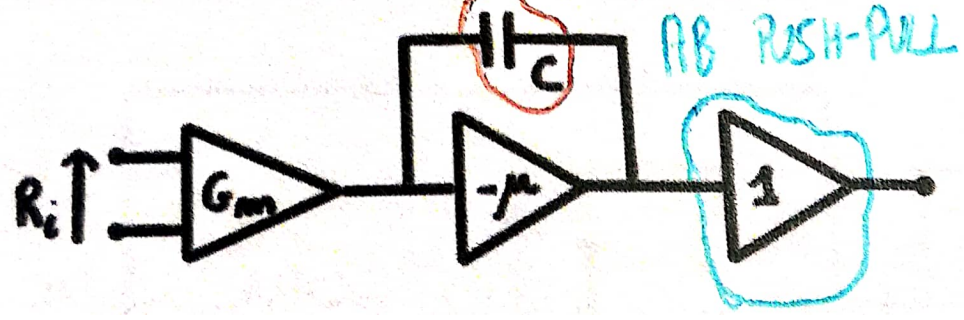
\includegraphics[scale=0.4]{Modello Semplificato.png}
\end{center}
\subsection{Non Idealità}
\textbf{Correnti di polarizzazione (DC)}\\
A causa della $R_{i}=\infty$, i morsetti hanno corrente idelmente nulla, ma questa è un'approssimazione, infatti lo stadio d'IN di un OPAMP è costituito da 2 transistor (è un differenziale) e quindi da 2 MOS/BJT, le quali basi assorbono un coorente di polarizzazione $I_{B}$.
Questa corrente di polarizzazione è data dalle correnti di bias:
\begin{equation}
    I_{B}=\frac{I_{B_{+}}+I_{B_{-}}}{2}
\end{equation}
La corrente di offset, invece, sarà la differenza delle correnti di bias:
\begin{equation}
    I_{B_{+}}-I_{B_{-}}
\end{equation}
\textbf{Slew Rate (AC)}\\
L'OUT di un OPAMP ideale può variare istantaneamente , passando da un valore all'altro in un tempo nullo.\\
L'OUT di un OPAMP reale, invece, varierà con velocità limitata (SR).\\
La $V_{OUT}$ cresce o diminuisce con pendenza sempre minore dello Slow Rate.
\subsection{Circuiti con OPAMP}
\textbf{Integratore}\\
Il circuito ha la stessa topologia dell'amplificatore invertente, quindi:
\begin{equation}
    A_{v}=\frac{v_{o}}{v_{i}}(s)=-\frac{Z_{2}(s)}{Z_{1}(s)}=-\frac{\frac{1}{sC}}{R}=-\frac{1}{sRC}
\end{equation}
o nel dominio del tempo:
\begin{equation}
    v_{o}(t)=-\frac{1}{RC}\int_{0}^{t}v_{i}(\tau)d\tau
\end{equation}
Come si può notare, questo circuito ha guadagno infinito in DC. Nel dominio del tempo, questo si traduce nel fatto che l'uscita aumenta indefinitivamente (fino alla saturazione) se l'ingresso ha una componente continua non nulla.\\
Questo è un problema perchè qualsiasi componente continua indesiderata nell'ingresso, o un offset nel circuito stesso, porta in breve tempo l'OPAMP alla saturazione.
Per ovviare a ciò, si usa un filtro passa basso con frequenza di taglio non nulla:
\begin{equation}
A_{v}=-\frac{\frac{R_{1}}{1+sR_{1}C}}{R_{1}}=-\frac{R_{1}}{R}\frac{1}{1+sR_{1}C}
\end{equation}
Quindi questa f.d.t. ha un polo a $\omega_{p}=\frac{1}{R_{1}C}$, invece che nell'origine, e questo permette un guadagno finito in DC \\\\
\textbf{Derivatore}\\
Anche questo circuito ha la stessa topologia dell'amplificatore invertente:
\begin{equation}
    \frac{v_{o}}{v_{i}}(s)=-\frac{Z_{2}(s)}{Z_{1}(s)}=-\frac{R}{\frac{1}{sC}}=-sRC
\end{equation}
oppure nel dominio del tempo:
\begin{equation}
    v_{o}(t)=-\tau\frac{dv_{i}}{dt}
\end{equation}
Il guadagno di questo circuito, tende all'infinito all'aumentare della frequenza, rappresentando il caso duale dell'integratore, il quale tendeva all'infinito al tendere della frequenza a zero.\\
In questo caso , il guadagno sempre più alto porta ad amplificare anche segnali non voluti, anche il rumore, tanto da poter saturare l'OPAMP.\\
Il rimedio a questo può essere trovato considerando che il guadagno aumenta perchè l'impedenza della C d'ingresso diminuisce all'aumentare della frequenza, tendendo idealmente a zero per frequenze infinite.\\
Porre una R in serie al C, pone un limite alla diminuzione del guadagno dell'OPAMP invertente:
\begin{equation}
    {v_{o}}{v_{i}}(s)=-\frac{R}{\frac{1}{sC}+R_{1}}=-\frac{sRC}{1+sR_{1}C}
\end{equation}
\newpage
\section{Oscillatori}
\textbf{Oscillatore di Gouriet-Clapp}\\
E' una variante dell'oscillatore di Colpitts in cui all'induttore è aggiunto in serie un condensatore.\\
Questo permette di modificare la frequenza di oscillazione mantenendo inalterato l'ammontare della retroazione, stabilita dal partitore fra le altre 2 capacità.\\
Questo circuito LC serie, ha un comportamento capacitivo (reattanza minore di zero) per pulsazioni minori della sua risonanza.\\
Quindi tale circuito risuonerà con i condensatori, $C_{1}$ e $C_{2}$, nell'intervallo di frequenze in cui manifesta un comportamento induttivo.\\
Per questo motivo è conveniente rappresentare il circuito LC serie come un'induttanza dipendente dall frequenza, da determinare calcolando la seguente impedenza serie:
\begin{equation}
    Z_{S}=sL+\frac{1}{sC_{0}}=s(L+\frac{1}{s^2C_{0}})=sL_{eq}(\omega)
\end{equation}
Ci siamo ricondotti all'oscillatore di Colpitts, la cui pulsazione di oscillazione è pari a:
\begin{equation}
    \omega_{0}^2=\frac{1}{L_{eq}C_{S}}=\frac{1}{(L-\frac{1}{\omega_{0}^2})C_{S}}
\end{equation}
Che può essere scritta come:
\begin{equation}
     \omega_{0}^2L-\frac{1}{C_{0}}=\frac{1}{C_{S}}=\frac{1}{C_{1}}+\frac{1}{C_{2}}
\end{equation}
Ovvero
\begin{equation}
    \omega_{0}=\sqrt{\frac{1}{L}(\frac{1}{C_{0}}+\frac{1}{C_{1}}+\frac{1}{C_{2}})}
\end{equation}
Cioè la frequenza di oscillazione è determinata da L e dalla serie delle tre capacità.\\\\
\textbf{Oscillatori al Quarzo}\\
Analizzo l'impedenza RLC:
\begin{equation}
    Z(s)=\frac{s^2+s\frac{R}{L}+\omega_{S}^2}{sC_{P}(s^2+s\frac{R}{L}+\omega_{P}^2)}=\frac{s^2+2\zeta\omega_{s}s+\omega_{s}^2}{sC_{P}(s^2+2\zeta\omega_{s}s+\omega_{P}^2)}
\end{equation}
dove le due pulsazioni valgoni rispettivamente:
\begin{equation}
    \omega_{S}=\frac{1}{\sqrt{LC_{S}}}
\end{equation}
\begin{equation}
    \omega_{P}=\frac{1}{\sqrt{L\frac{C_{S}C_{P}}{C_{S}+C_{P}}}}
\end{equation}
\newpage
\noindent
Inizio a studiare la fase:\\
Siccome so che la $\zeta$ è molto bassa, avrò 2 zeri complessi coniugati alla frequenza di risonanza $\omega_{S}$, 2 poli complessi e coniugati alla frequenza $\omega_{P}$, ma $\omega_{S}\simeq\omega_{P}$ e un polo in zero (DC).\\
Quindi per qualsiasi frequenza maggiore di 0, avrò una fase pari a $\phi=-\frac{\pi}{2}$.\\
Tra gli zeri e i poli, chi è più bassa (chi ha prima effetto)? La serie tra $C_{P}$ e $C_{S}$ è minore di $C_{S}$, quindi la $\omega_{P}$ sarà più alta.\\
Arriveranno, quindi prima gli zeri complessi e coniugati, con un'attenuazione bassa (variazione veloce), i quali mi faranno ruotare la fase di $\pi$.
Poi arrivano i poli, con le stesse caratteristiche, quindi altrettanto velocemente i poli mi riportano la fase a $-\frac{\pi}{2}$.
Quello che mi interessa di più è che la fase tra $\omega_{S}$ e $\omega_{P}$, la fase vale $\frac{\pi}{2}$, proprio come un INDUTTORE !!!
\begin{center}
    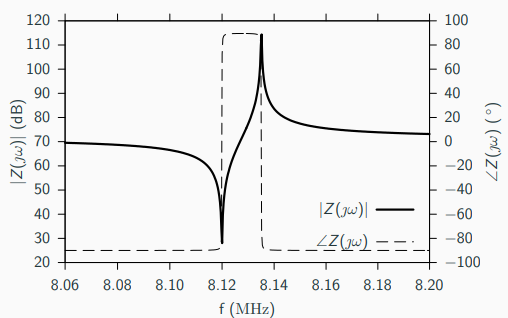
\includegraphics[scale=0.8]{Quarzo.png}
\end{center}
\vspace{0.4mm}
\textbf{Oscillatori di Rilassamento}\\
Per ottenere un circuito con punto di equilibrio instabile, serve un circuito generico caricato da un bipolo non lineare, con un tratto a $R<0$ e 2 tratti a $R>0$
\\\\
\textbf{Oscillatori di Rilassamento con Bipoli Comandati in Corrente}\\
Supponiamo di avere un bipolo che manifesta un tratto a $R<0$
\begin{equation}
    \frac{di}{dt}=-\frac{1}{Cf'(i)}(i-I_{0})
\end{equation}
Voglio ora andare a studiare il segno della derivata, il quale è composto da 3 parti:
\begin{enumerate}
    \item Il segno $-$
    \item Il segno di $f'(i)$
    \item Il segno di $(i-I_{0})$
\end{enumerate}
\newpage
I punti da prendere in considerazione sono $i_{12}$, $I_{0}$ e $i_{21}$:
\begin{enumerate}
    \item Per \textbf{$i<i_{12}$} ho $f'(i)>0$ e $i-I_{0}<0$ quindi $\frac{di}{dt}>0$ (la corrente aumenterà)
    \item Per \textbf{$i_{12}<i<I_{0}$} ho $f'(i)<0$ e $i-I_{0}<0$ quindi $\frac{di}{dt}<0$
      \item Per \textbf{$I_{0}<i<i_{21}$} ho $f'(i)<0$ e $i-I_{0}>0$ quindi $\frac{di}{dt}>0$
      \item Per \textbf{$i>i_{21}$} ho $f'(i)>0$ e $i-I_{0}>0$ quindi $\frac{di}{dt}<0$ (la corrente diminuirà)
\end{enumerate} 
Le frecce mi indicano come vengono percorse le caratteristiche nel tempo.\\
In DC, $i=I_{0}$ è il punto di equilibrio. Anche una minima perturbazione (rumore) porterà la corrente ad assumere valore maggiori o minori del punto di equilibrio (instabile).\\
Partendo, ora, dall'origine, la $I_{0}$ mi inizia a caricare C finchè la tensione non varrà $V_{2}$ (es. tensione che fa accendere la lampadina). Da $V_{2}$ faccio un salto al secondo tratto a resistenza positiva, perchè non posso scendere sul tratto a resistenza negativa.\\
Occhio però, non è un salto istantanea, perchè $i_(t)$ deve essere continua.\\
Ora il consensatore dovrà scaricarsi, quindi scenderò fino a $V_{1}$ e salto sul primo tratto.\\
Mi ritroverò come prima, in un ciclo limite!!!
\begin{center}
    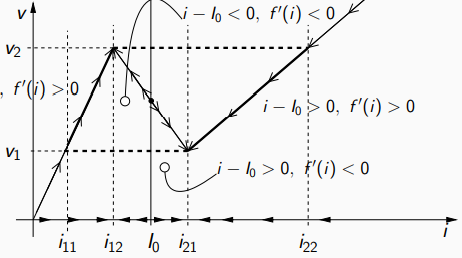
\includegraphics[]{Derivata.png}
\end{center}
Abbiamo studiato il segno della derivata, ora la risolvo per trovare la i in funzione del tempo:\\
Faccio un cambio di variabile: $i'=i-I_{0}$\\
\begin{equation}
    \frac{di'}{dt}=-\frac{i'}{Cf'(i)}
\end{equation}
Se f'(i) è lineare a tratti, la f'(i) sarà una costate (assumerà un valore diverso in ognuna delle regioni di funzionamento).\\
Inoltre $f'(i)$, oltre ad essere una costante, è la derivata di v fatta rispetto ad i, quindi una resistenza ($R\uparrow$ e $R\downarrow$ entrambe positive e con le frecce per discriminare il tratto che si sta percorrendo.)\\
Avrò quindi 2 equazioni differenziali:
\begin{equation}
    \frac{di'}{dt}=-\frac{i'}{CR\uparrow}
\end{equation}
\begin{equation}
    \frac{di'}{dt}=-\frac{i'}{CR\downarrow}
\end{equation}
$R\uparrow$ e $R\downarrow$ sono l'accelerazione della corrente.
La soluzione di queste 2 equazioni è:
\begin{equation}
    i'(t)=i(0)(e^(-t/(CR\updownarrow)))
\end{equation}
\begin{equation}
    i(t)=(i(0)-I_{0})e^(-t/(CR\updownarrow))+I_{0}
\end{equation}
Dalla quale ricavo:
\begin{equation}
    v=R\updownarrow i(t)
\end{equation}
$i(0)$ sarà alternativamente $i_{22}$ o $i_{11}$ e le traiettorie saranno valide fino al raggiungimento dei valori $i_{21}$ e $i_{12}$.
\newpage
\section{Stadi di Uscita}
\textbf{Classe A - Push Pull}\\
Al posto del generatore di corrente ci metto 2 transinstor complementari, npn e pnp.\\
$V_{BB}$ è una tensione costante DC \\
Facendo la KVL ottengo:\\
\begin{equation}
    v_{BE}+v_{EB}=V_{BB}
\end{equation}
Dal momento che la somma è costante, se aumento $v_{BE}$, dovrò diminuire $v_{EB}$ e viceversa.\\
Facendo ora i piccoli segnali, ottengo: \\
\begin{equation}
    v_{be}+v_{eb}=0
\end{equation}
Quindi se la corrente di collettore, aumenta, perchè aumenta la $v_{BE}$, diminuirà la $v_{EB}$. Quindi le due correnti procedono in opposizione di fase, entrambe con un valor medio sempre diverso da 0 !!! (vedi figura)\\
Se mi vado a calcolare il rendimento, sarà uguale a quello di prima; cambierà il rendimento massimo.\\
\begin{equation}
    \eta=\frac{\hat{v_{O}}^2}{2R_{L}}\frac{1}{2V_{DD}I_{C}}
\end{equation}
Analizzando il nodo, otterrò $i_{L}(t)=i_{C_{n}}-i_{C_{p}}$, ma come ampiezza, otterrò la somma delle 2 ampiezze: 
\begin{equation}
    \hat{i_{L}}=\hat{i_{C_{n}}}+\hat{i_{C_{p}}}=2\hat{i_{C}}
\end{equation}
\begin{equation}
    \hat{v_{O}}=\hat{i_{L}}R_{L}=2\hat{i_{C}}R_{L}
\end{equation}
La minima $I_{C}$ necessaria al mantenimento del transistor nella regione attiva dovrà essere:
\begin{equation}
    I_{C}=\hat{i_{C}}
\end{equation}
Sostituendo l'equazione trovata prima, ottengo:
\begin{equation}
    I_{C}=\hat{i_{C}}=\frac{V_{DD}}{2R_{L}}
\end{equation}
Mi basta sostituire e il risultato sara che $ \eta=50\% $.
\begin{center}
    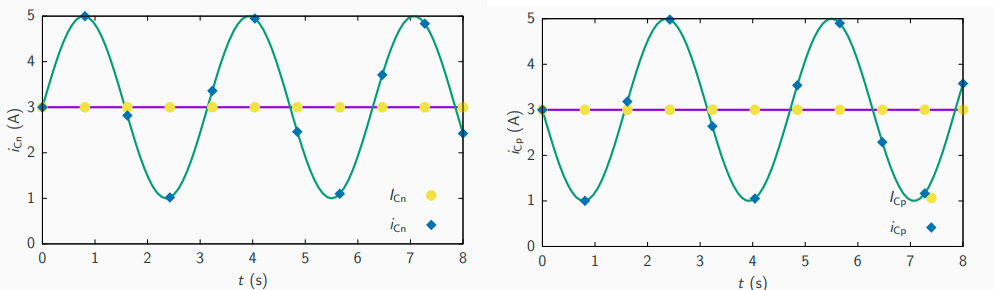
\includegraphics[scale=0.6]{Exit.png}
\end{center}
\end{document}


